\section{Introducción}

\subsection{1.1 Motivación y contexto ambiental}

Frente al acelerado deterioro de los ecosistemas planetarios, las redes de sensores distribuidos emergen como herramienta indispensable para capturar datos ambientales en tiempo útil. Particularmente llamativo resulta cómo la integración de constelaciones en órbita baja (LEO) con sensores IoT de bajo consumo abre posibilidades antes inalcanzables para el monitoreo continuo de variables críticas como temperatura, humedad del suelo, calidad del aire o niveles de biodiversidad. 

Aunque las constelaciones LEO ofrecen cobertura global y latencia reducida en comparación con sistemas GEO tradicionales, su verdadero potencial en aplicaciones ambientales radica en la capacidad de establecer enlaces directos con sensores remotos desplegados en zonas de difícil acceso. Shayea et al. destacan precisamente esta convergencia entre IoT y redes LEO como uno de los pilares para infraestructuras de observación terrestre de próxima generación, especialmente en el contexto de evoluciones hacia 5G/6G \cite{Shayea2024}. 

Resulta revelador observar que muchos despliegues actuales aún dependen de arquitecturas de antena optimizadas para comunicaciones satelitales generales, sin un enfoque específico en las demandas únicas del monitoreo ambiental distribuido. Un ejemplo concreto lo constituye el desarrollo de antenas helicoidales L/S desplegables integradas en CubeSats para observación terrestre, que demuestran ganancias elevadas y buen comportamiento en entornos operativos reales \cite{Meirambekuly2023}.

\begin{table*}[htbp]
\renewcommand{\arraystretch}{1.3} % Mantiene el espaciado vertical limpio de IEEE
\centering
\caption{\textsc{Comparación de Características Principales entre Bandas L y S para Enlaces LEO-IoT Ambientales}}
\label{tab:bandas_l_s}
% \columnwidth fuerza a que la tabla mida exactamente el ancho de la columna actual
\begin{tabularx}{\columnwidth}{|X|c|c|}
\hline
\textbf{Parámetro} & \textbf{Banda L} & \textbf{Banda S} \\ \hline
Frecuencia típica & 1-2 GHz & 2-4 GHz \\ \hline
Penetración atmosférica & Excelente & Buena \\ \hline
Ancho de banda disponible & Moderado & Mayor \\ \hline
Tamaño de antena requerido & Mayor & Menor \\ \hline
Sensibilidad a Doppler & Menor & Moderada \\ \hline
\end{tabularx}
\end{table*}

\subsection{1.2 Desafíos de comunicación LEO-IoT}

Uno de los desafíos persistentes que surge al analizar estas arquitecturas radica en la naturaleza altamente dinámica de los enlaces LEO. El movimiento relativo a gran velocidad genera desplazamientos Doppler significativos, variaciones rápidas de canal y ventanas de visibilidad limitadas, condiciones que afectan particularmente a sensores de bajo consumo energético desplegados en entornos remotos.

Lejos de ser un asunto resuelto, la literatura reciente sugiere que el diseño de la antena se convierte en el elemento crítico que determina la viabilidad completa del sistema. Diseños que logran combinar ganancia suficiente, polarización circular robusta y patrones de radiación adecuados tienden a mitigar mejor estos efectos. No obstante, cabe matizar que muchos enfoques optimizados para comunicaciones de datos de alta velocidad muestran limitaciones cuando se aplican a flujos intermitentes y de baja tasa de sensores ambientales.

\begin{figure}[h]
\centering
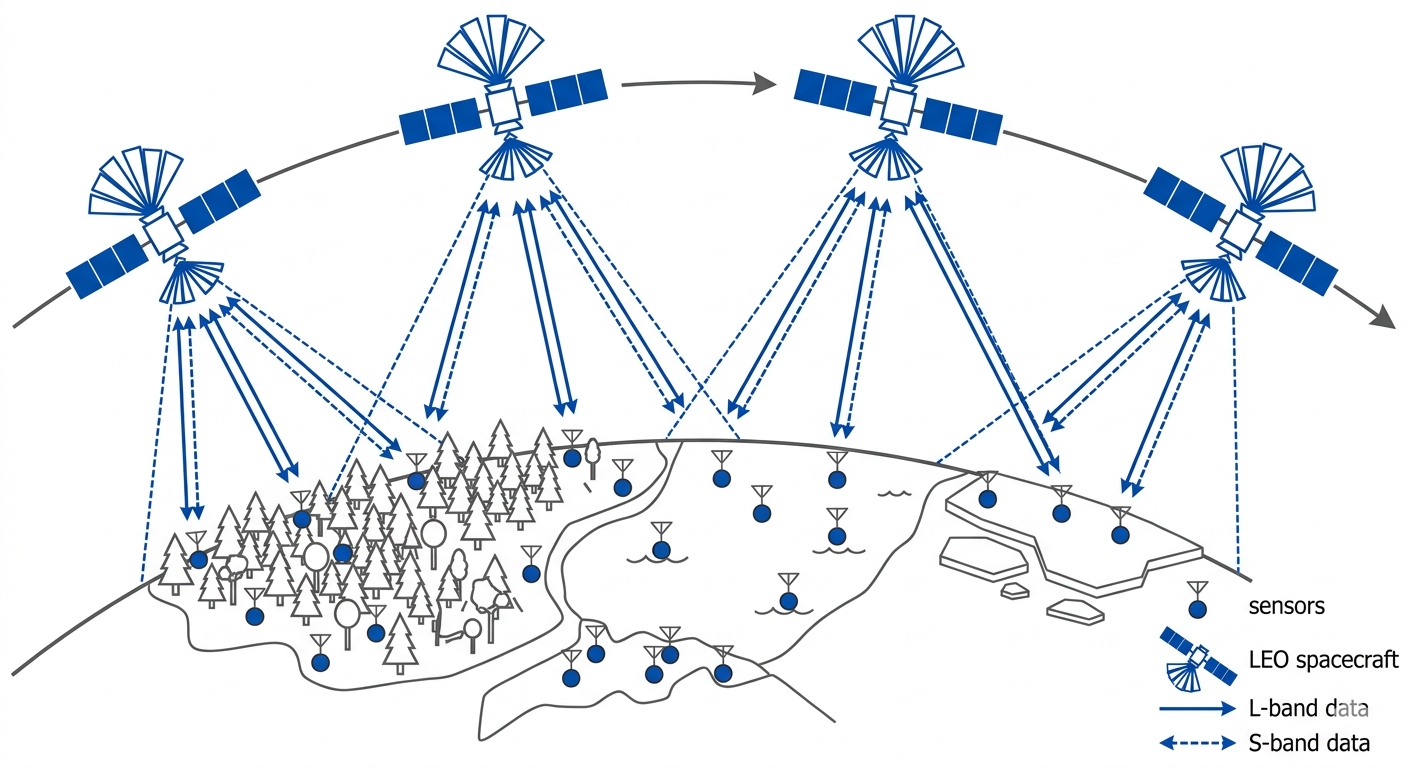
\includegraphics[width=\linewidth]{fig1.png}
\caption{Escenario general de red de sensores ambientales conectada vía constelación LEO en bandas L/S, mostrando enlaces uplink/downlink, cobertura multi-satélite y nodos IoT distribuidos en terreno.}
\label{fig:general_scenario}
\end{figure}

\subsection{1.3 Objetivos de investigación}

Particularmente llamativo es el hecho de que, a pesar de los avances en plataformas CubeSat y phased-array, persisten brechas importantes en el análisis comparativo de arquitecturas de antena específicamente orientadas a gestión ambiental vía LEO. 

Este trabajo busca llenar parte de ese vacío mediante un análisis detallado de soluciones en bandas L y S. Los objetivos principales incluyen evaluar el rendimiento de distintas arquitecturas (conformes, helicoidales desplegables y phased-array), identificar trade-offs relevantes para aplicaciones de sensores ambientales y proponer recomendaciones de diseño que maximicen cobertura y eficiencia energética. Guler et al. ilustran bien el potencial de arrays conformes en escenarios LEO dinámicos, sirviendo como referencia para el análisis comparativo que desarrollaremos \cite{Guler2025}.

Las secciones siguientes presentan primero el estado del arte, luego los requisitos de sistema, el análisis de arquitecturas, resultados de evaluación, discusión de implicaciones y, finalmente, conclusiones con líneas de trabajo futuro.